\chapter{General Collective Behavior Algorithm Applications to Passive FM Radar}
\label{chapter:passive}
\thispagestyle{myheadings}

\graphicspath{{Passive/}}

Note: the code developed for this chapter is in \citet{cviono}.

\section{Passive Hitchhiker Radar Background}

MIT Haystack and the University of Washington have been at the forefront of passive radar ionospheric research over the past two decades with the ISIS distributed passive hitchhiker radar instrument.  
A primary geospace target for ISIS is detection of ionospheric turbulence.
Such turbulence, detectable by backscattered broadcast signals \citep{willisbook} can disrupt waves traveling through the ionosphere up to about \unit[2]{GHz}, which includes life-critical navigation services such as GPS and aircraft satellite transponders. 
A dominant scattering mechanism of these ionospheric turbulences is thought to be Bragg scatter, the effects of which have also manifested in ISR spectrum covered in this dissertation. 
Following the development in \citet{sahr2007}, we define an incident quasi-monochromatic wavevector $k_i$ coming from the FM transmitter $x(t)$. 
Using the assumption that only longitudinal $B_\parallel$ ion-acoustic density waves yield significant scatter \citep{stromme2006,sahr2007,thide1990}, then the scattered wavevector $k_s=-k_i$ and phonon region wavenumber $k_p$ are related by 
\begin{equation}
k_i = k_p + k_s \leftrightarrow k_i = k_p - k_i \leftrightarrow 2 k_i = k_p 
\end{equation}
Observe that 
\begin{equation}\label{eq:abragg}
k = \frac{2\pi}{\lambda} \rightarrow \frac{1}{2\lambda_i} = \lambda_p
\end{equation}
which is representative of classical Bragg scatter. 
\eqref{eq:abragg} means in simple terms that a coherent or incoherent radar will detect only scattering at a wavelength \nicefrac{1}{2} that of the incident radar waveform $x(t)$. 
A \unit[100]{MHz} FM transmitter signal of wavelength \unit[3]{m} will yield Bragg scatter from ion-acoustic waves with wavelength \unit[1.5]{m}. 
By inspection we see it is useful to have radars with a wide variety of incident wavenumbers. 
The ISIS system and upcoming passive radar systems such as RAPID \citep{lind2015} cover the \unit[50]{MHz} to \unit[650]{MHz} range and so should be useful for coherent ionospheric returns at a variety of wavenumbers, unlike traditional ionospheric radar that are limited to a small percentage bandwidth frequency range.

Better characterization of such turbulent events requires extended data collection. Since we do not know \textit{a priori} when or where such events are occurring, we cannot count on incoherent radar scatter (ISR) sites alone to provide the desired data volume. 
Since the passive receiver antennas have a relatively broad beamwidth \citep{lind2013}, the only time limitation is hard drive space.
Data storage was a nearly crippling factor in the 1990s \citep{sahr1997}) but has become more tractable with technology advances. 
Increasing receiver bandwidths and the desire to use multistatic configurations brings the datastream bandwidth up to challenging levels again--necessitating data pruning and curation at an early stage. 

Until recently, only a few \unit[150]{kHz} segments of the FM broadcast spectrum could be simultaneously captured \citep{lind2013}. 
Storage and sharing of data has been problematic due to limitations in instrument site storage, processing, and network bandwidth.  
All three barriers have been pushed down with \$130 USB 3.0 4TB hard drives with sustained sequential \unit[100]{MB/s} read/write speeds, powerful quad-core \$500 desktop PCs, and nearly-ubiquitous \unit[50]{Mbps} Internet connections. 
The RF receivers themselves have markedly improved, with recent COTS models allowing \unit[1]{GHz} streaming bandwidth \citep{lind2015} versus the \unit[2]{MHz} streaming bandwidth previously used in the ISIS instrument.

Given the increasing data collection rate due to additional sites and broader RF bandwidth, the need for automated target detection is increasingly urgent not only for ISIS, but for other passive radar instruments. 
The larger the data bandwidth, the larger the need to prune the data early for relevant events due to limited HDD resources. 
Inexpensive desktop PCs are capable of on-line target detection, written in straightforward Python script. 
We use a blind machine vision process that does not require human algorithm “training” or extensive fiddling with parameters. 
Initial values were heuristically chosen, followed by minor empirically-based adjustments. 
We found empirically that some data has highly unstable cross-ambiguity functions with signal to clutter ratio (SCR) varying over the entire dataframe (range-Doppler plot) by several orders of magnitude in a non-stationary way. 
Such variations would be vexing to a standard machine vision algorithm. 
A future pathway to better exploiting these data intermixed with sporadic bad data may be on-line qualification of dataframes by measured self-ambiguity of the reference signal.

\section{Algorithm}

In this chapter, computer vision techniques are applied to 2D range-Doppler maps. 
For convenience and consistency, we will refer to the 2D range-Doppler map from a single incoherent integration interval (e.g. 2, 5, or 10 seconds) as a ``dataframe.'' 
A simplified view of the overall process is shown in Figure~\ref{fig:fmgenalgo}.
\begin{figure}\centering
    %the \par is necessary after each text to make the \baselineskip take effect
    \begin{tikzpicture}[node distance=1.5cm, auto]

    \node (in) [startstop,text width=2cm] {streaming data frames \par};

    \node (detect) [compute, right of=in,text width=3.5cm,xshift=2cm] { Detect Ionospheric Turbulence \par };

    \node (reduce) [process, right of=detect, text width=3cm,xshift=2.5cm] { Parameter Extraction \par };


    \draw[arrow] (in) -- (detect);
    \draw[arrow] (detect) -- (reduce);

    \end{tikzpicture}

    \caption{Block diagram of general passive hitchhiker radar ionospheric turbulence detection algorithm.}
    \label{fig:fmgenalgo}
\end{figure} 
A more detailed view of the preliminary machine vision algorithm for each pixel is presented in Figure~\ref{fig:fmblock}.
\begin{figure}\centering 
    %the \par is necessary after each text to make the \baselineskip take effect
    \begin{tikzpicture}[node distance=1.5cm, auto]
    
    \node (in) [startstop,text width=2.5cm] {Load next image};
    
    \node (filt) [process, below of=in,text width=2cm] { Wiener filter \par };
 
    \node (gmm) [compute, below of=filt,] { GMM \par };

	\node (erode) [compute, below of=gmm,text width=3cm] { Morphological Erosion \par};
    \node (dilate)[compute,below of=erode,text width=3cm] { Morophlogical Dilation \par};
    
    \node (conn) [compute,below of=dilate,text width=3cm] { Connected Components \par};
    
    \node (loc) [startstop,below of=conn,text width=4cm] { Location and Extent of Turbulence \par};
    
    \draw[arrow] (in) -- (filt);
    \draw[arrow] (filt) -- (gmm);
    \draw[arrow] (gmm) -- (erode);
    \draw[arrow] (erode) -- (dilate);
    \draw[arrow] (dilate) -- (conn);
    \draw[arrow] (conn) -- (loc);
    \end{tikzpicture}
    
    \caption{Passive hitchhiker radio computer vision algorithm for detecting ionospheric turbulence.}
    \label{fig:fmblock}
\end{figure}

Wiener filtering has been described in section~\ref{sec:filtnoise}.
After filtering, the dataframes pass to the main turbulence discrimination algorithm.

\subsection{Segmentation: Gaussian Mixture Method}

Originally reported by \citet{stauffer1999}, the Gaussian Mixture Method (GMM) is a dense algorithm used to distinguish to which of several Gaussian distributions the current pixel value belongs to.
For example, assume that background noise may be modeled with Gaussian pdf $N(\mu_1,\sigma_1)$, and that ionospheric turbulence follows Gaussian pdf $N(\mu_2,\sigma_2)$ and airplanes and meteors follow $N(\mu_3,\sigma_3), N(\mu_4,\sigma_4)$ and so on as illustrated in Figure~\ref{fig:gmm}.
\begin{figure}\centering
    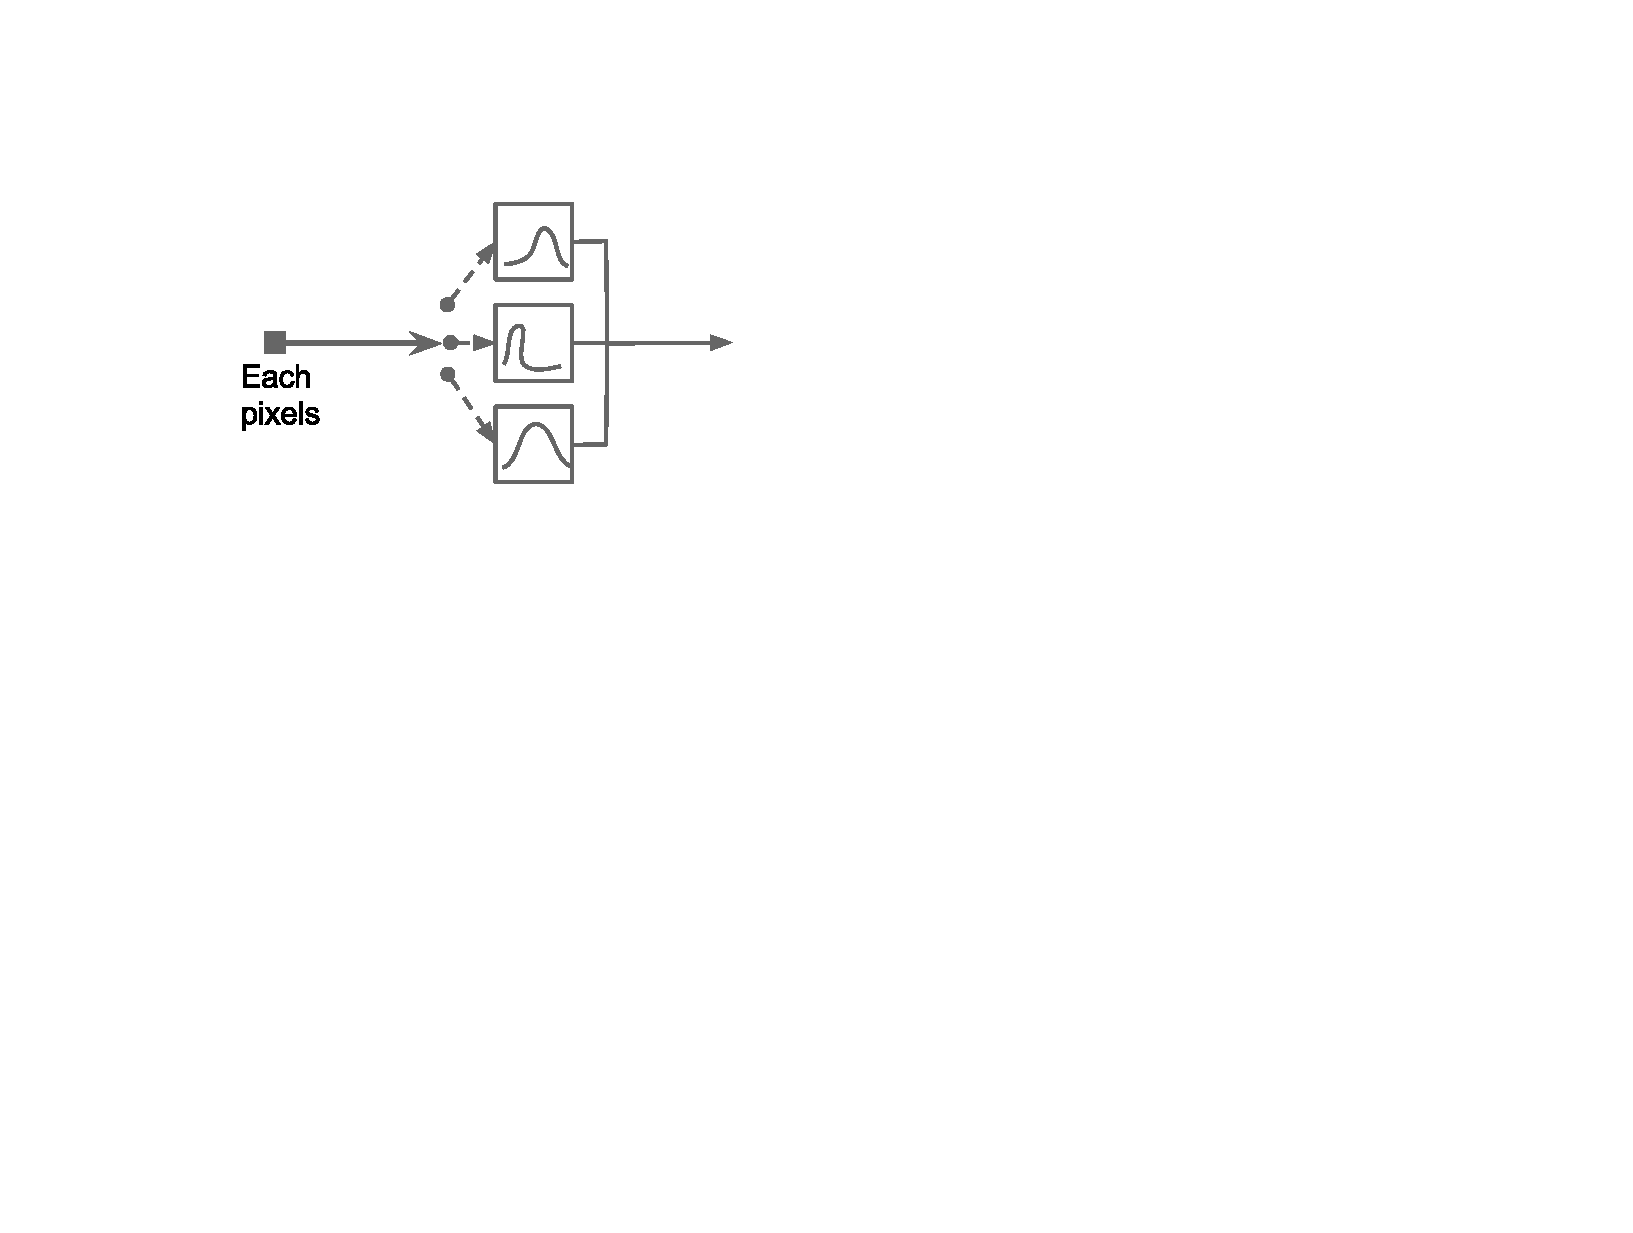
\includegraphics[width=0.8\linewidth,trim=60 350 420 80,clip]{gfx/gmm}
    \caption{GMM examples of three distributions, where the output is the confidence of pixel value to each distribution.}\label{fig:gmm}
\end{figure}
Typically GMM implementations experience a few false positives, particularly for non-stationary noise, which are manifested as isolated pixels falsely declared as foreground.
Example GMM output using actual ISIS data is depicted in Figure~\ref{fig:gmmout}.
\begin{figure}\centering
    \includegraphics[width=\linewidth]{gfx/gmmout}
    \caption{GMM algorithm binary output (white desired) on actual ISIS range-Doppler dataframe}\label{fig:gmmout}
\end{figure}
The result clearly needs further processing; morphological algorithms are implemented.

\subsection{Morphological Erosion}
Morphological erosion is a set process in which a structuring element (SE), in this case a disk 3 pixels in diameter, is passed over each pixel in Figure~\ref{fig:gmmout}.
The erosion algorithm is described in section~\ref{sec:erode}.
For the data from Figure~\ref{fig:gmmout}, erosion results in Figure~\ref{fig:erodeout}.
\begin{figure}\centering
	\includegraphics[width=\linewidth,trim=0 20 0 20,clip]{gfx/erodeout}
	\caption{Erosion processed data with 3 pixel disk structuring element. Desired pixels in white. Turbulence has been isolated from clutter.}\label{fig:erodeout}
\end{figure}
The turbulence has been well-isolated from the clutter in Figure~\ref{fig:erodeout}.
However, the desired convex hull of pixels representing the actual ion-acoustic turbulence return have been eroded down to the point that connected components analysis will miss the associations of nearby pixels and declare a false negative--that no ionospheric turbulence existed here. 
The turbulence regions are reassociated by performing morphological dilation.

\subsection{Morphological Dilation}
Morphological dilation is a set process in which a structuring element is passed over pixel regions. 
Dilation is described in section~\ref{sec:dilate}.
For passive FM radar data, dilation is used to join associated regions of ionospheric turbulence in the processing of real passive radar data. 
The morphological dilation of actual data using a disk structuring element of diameter 5 pixels is shown in Figure~\ref{fig:dilateout}. 
\begin{figure}\centering
    \includegraphics[width=\linewidth,trim=0 20 0 20,clip]{gfx/dilateout}
    \caption{Dilation processed data with 5 pixel disk structuring element. Desired pixels in white. Artificial gaps have been filled in by dilation.}\label{fig:dilateout}
\end{figure}
After associated pixel regions of the ionospheric returns have been rejoined the dataframe is ready for connected component blob analysis.


\subsection{Connected Component Analysis}
To make a final declaration on ionospheric turbulence candidates, we consider whether a region of sufficient associated pixel extent in the range-Doppler space is observed. 
This will exclude events less than a user-defined space and Doppler extent. 
A future algorithmic extension would exploit the time dimension via Kalman filtering to better positively classify small-scale ionospheric turbulence. 
The connected component algorithm is described in section~\ref{sec:blob}.
Large self-ambiguity shifts occur for large changes in broadcast signal entropy--for example on a rock music station during DJ announcements or a brief quiet period during song transitions. 
An example CCA for real data is shown in Figure~\ref{fig:ccaout}.
\begin{figure}
    \includegraphics[width=\linewidth]{gfx/ccaout}
    \caption{CCA target detection inside green box. Color represents signal to clutter ratio.}
    \label{fig:ccaout}
\end{figure}
The green box neatly highlights the detected ionospheric turbulence. 
Parameters of the turbulence (Doppler centroid--average velocity and range) can be directly estimated from the CCA bounding box characteristics.

\subsection{Real data analysis}
Several data frames are shown in Figure~\ref{fig:gmmdump} as an example of performance on real-world data. 
The code \citet{cviono} was forwarded to the MIT Haystack research for implementation on existing ISIS data and for the RAPID system in testing.
Initial results have shown adequately low Type I and Type II errors, with further improvement possible by tracking behavior through space and time instead of time only.
\begin{figure}\centering
    \begin{subfigure}[t]{0.45\linewidth}
        \includegraphics[width=\linewidth]{gfx/out-000}	
        \caption{23:14:59 two turbulent regions detected.}
    \end{subfigure}
    \quad
    \begin{subfigure}[t]{0.45\linewidth}
        \includegraphics[width=\linewidth]{gfx/out-001}
        \caption{23:15:09 one turbulent region detected.}
    \end{subfigure}
    \begin{subfigure}[t]{0.45\linewidth}
        \includegraphics[width=\linewidth]{gfx/out-002}
        \caption{23:15:19 one large turbulent region detected.}
    \end{subfigure}
    \begin{subfigure}[t]{0.45\linewidth}
        \includegraphics[width=\linewidth]{gfx/out-003}
        \caption{23:15:29 two adjacent turbulent regions detected.}
    \end{subfigure}
\end{figure}
\begin{figure}\ContinuedFloat \centering
    \begin{subfigure}[t]{0.45\linewidth}
        \includegraphics[width=\linewidth]{gfx/out-004}
        \caption{23:15:39 one turbulent region detected.}
    \end{subfigure}
    \begin{subfigure}[t]{0.45\linewidth}
        \includegraphics[width=\linewidth]{gfx/out-005}
        \caption{23:15:49 two small turbulent regions detected.}
    \end{subfigure}
    \caption{Real data sequence from Aug 3, 2010. Ionospheric turbulence detections enclosed in green boxes.}
    \label{fig:gmmdump}
\end{figure}
